\documentclass[handout]{beamer}
\usepackage{beamerthemesplit}
\usepackage{pgfpages}
\usepackage{verbatim}

\usepackage{tikz}
\usetikzlibrary{arrows,%
                shapes,positioning}

\tikzstyle{vertex}=[circle,fill=black!25,minimum size=20pt,inner sep=0pt]
\tikzstyle{selected vertex} = [vertex, fill=red!24]
\tikzstyle{edge} = [draw,thick,-]
\tikzstyle{weight} = [font=\small]
\tikzstyle{selected edge} = [draw,line width=5pt,-,red!50]
\tikzstyle{ignored edge} = [draw,line width=5pt,-,black!20]

\newcommand{\field}[1]{\mathbb{#1}} %requires amsfonts

\usetheme{Antibes}
\usecolortheme{beaver}
\title[Fast Software Encryption 2012 - Paper Review]{Fast Software Encryption 2012}

\usepackage{mathptmx}
\usepackage[scaled=.90]{helvet}
\usepackage{courier}
\usepackage[T1]{fontenc}

%%\pgfpagesuselayout{4 on 1}[letterpaper,border shrink=5mm]

\institute[RIT]{}
\date{\today}
%\subtitle{}
\author{Christopher A. Wood}
%\institute[]{}
%\date{}
\begin{document}

%%%%%
%%
%% Resource link: http://www.math-linux.com/spip.php?article77
%%
%%%%

\begin{frame}
	\titlepage
\end{frame}

\begin{frame}
	\frametitle{Agenda}
	\tableofcontents
\end{frame}

\section{Cryptographic algorithm security fundamentals}

%\begin{frame}
%	\frametitle{Chaos in the Logistic Map}
%	\begin{center}
%     		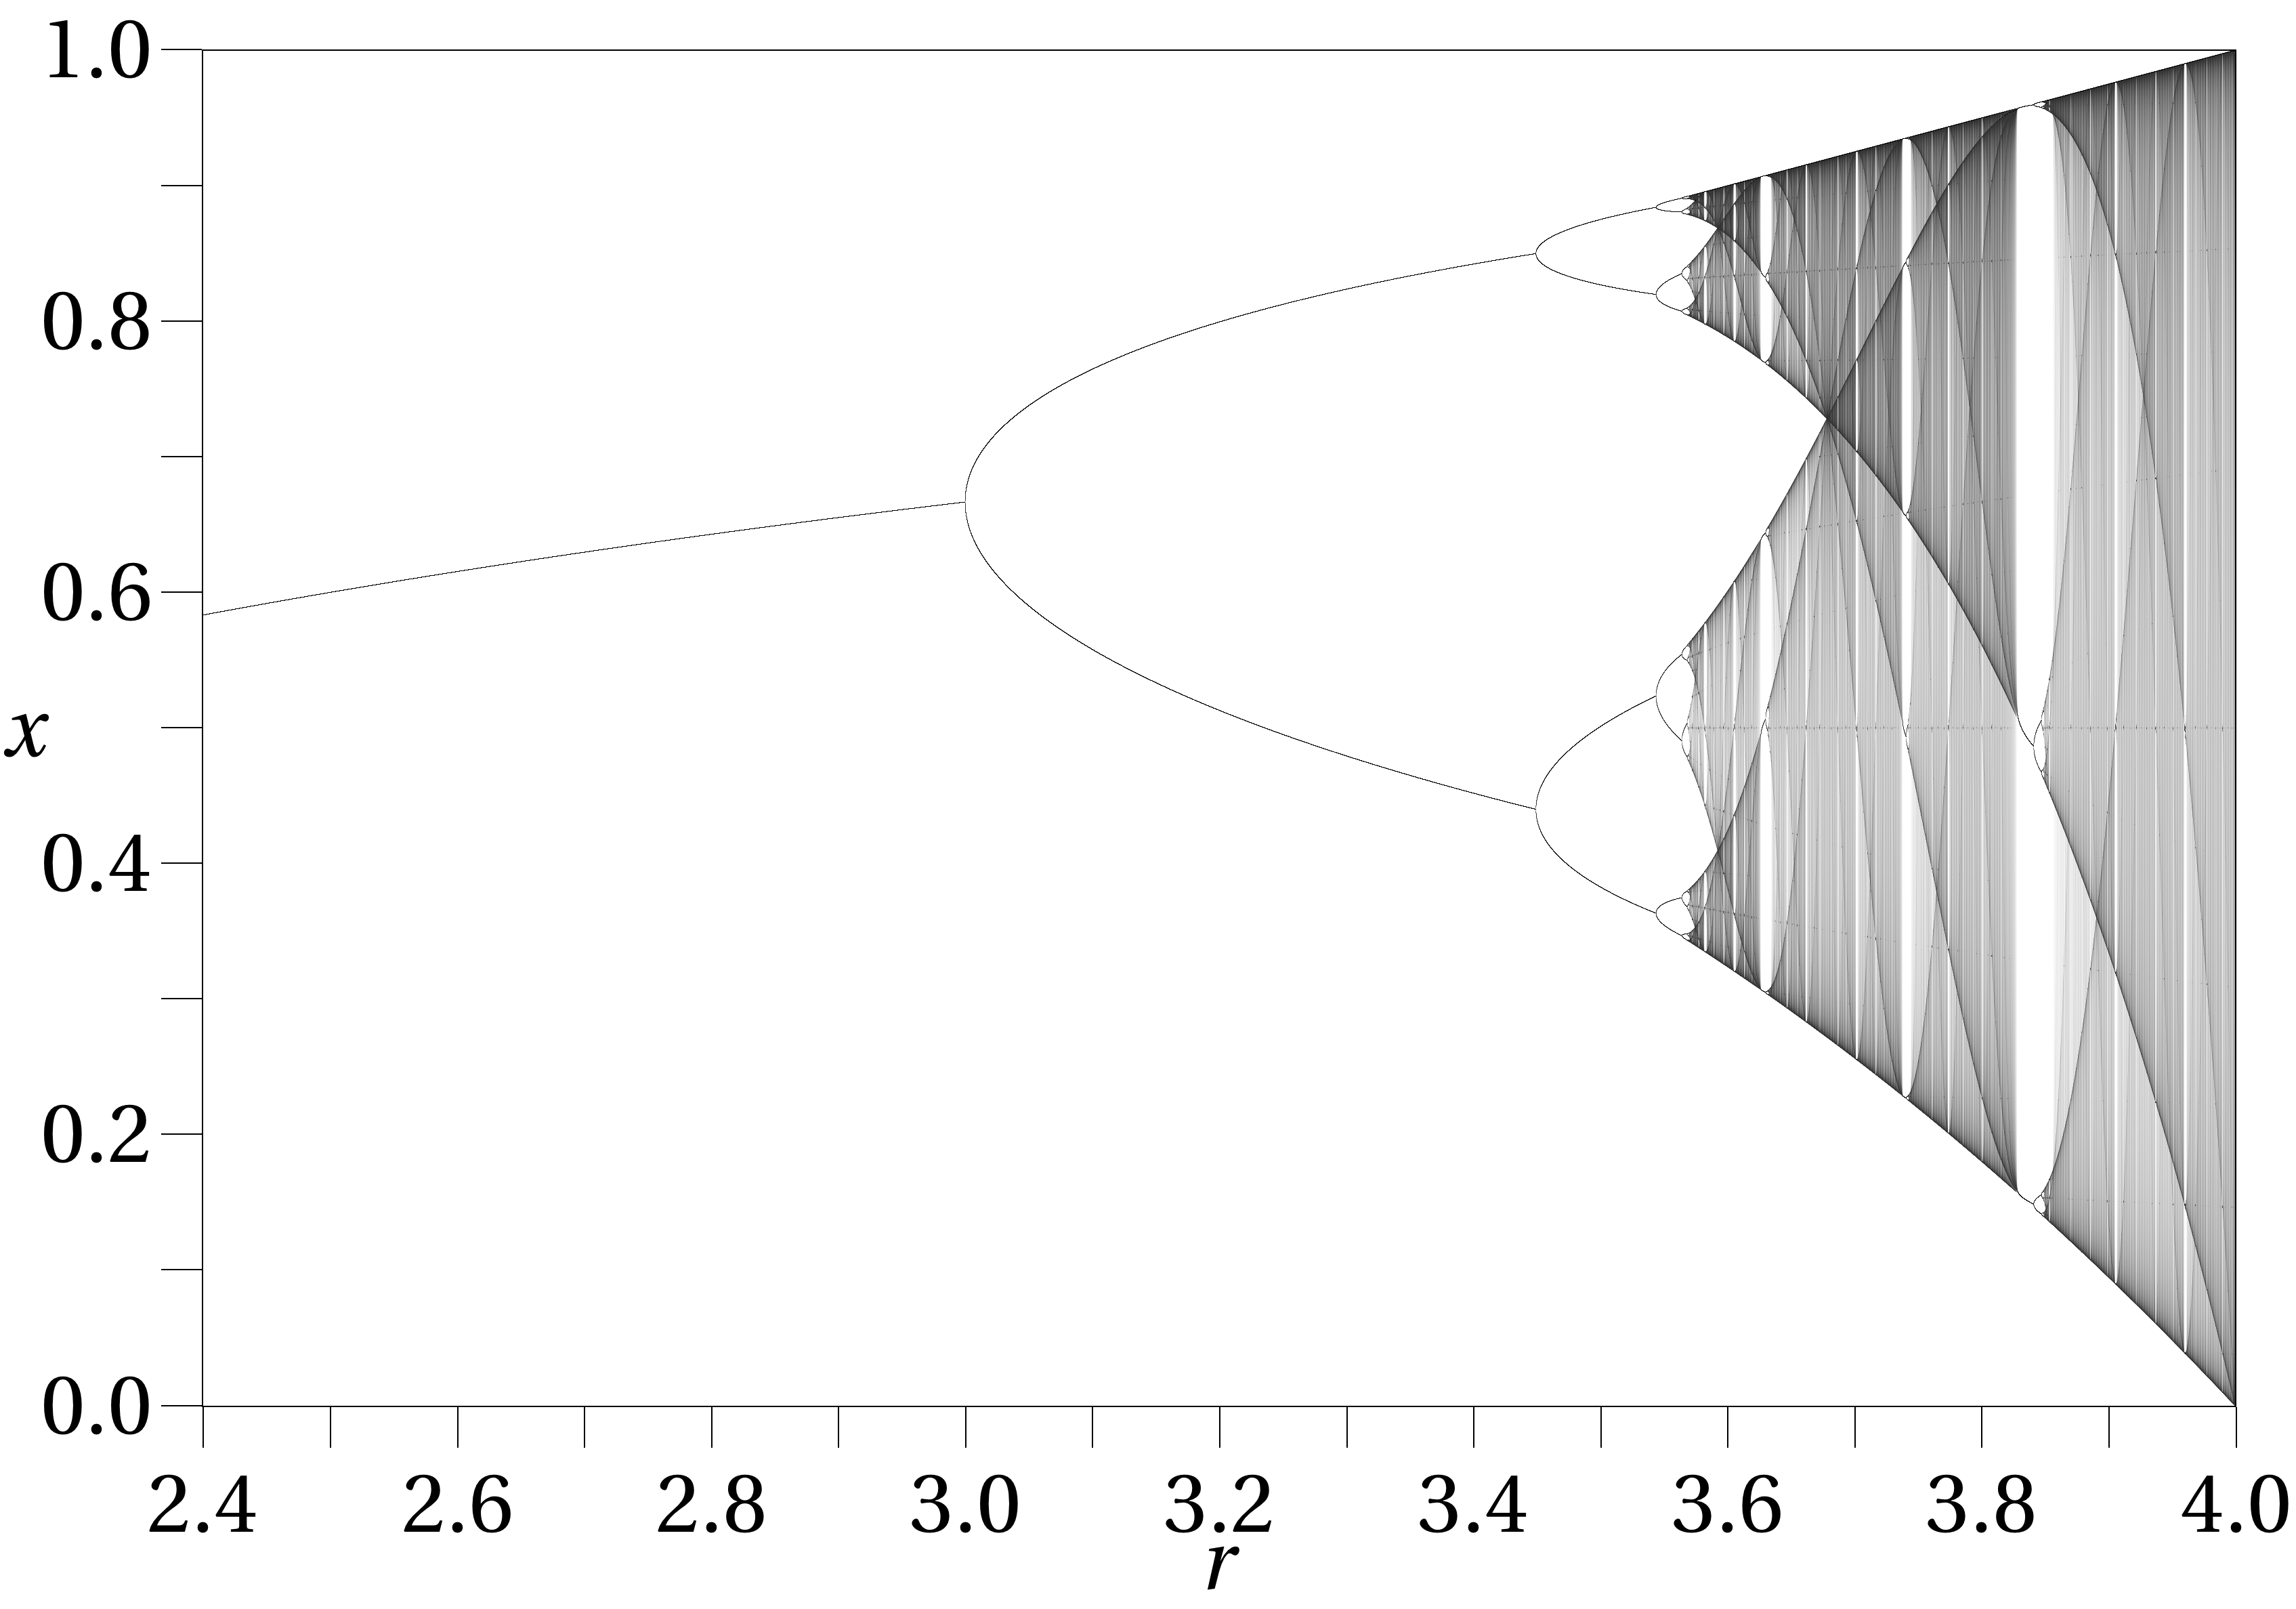
\includegraphics[width=90mm]{images/logistic_bifurcation.png}
%	\end{center}
%\end{frame}

\end{document}